\documentclass{scrartcl}

\usepackage{amssymb}
\usepackage{amsmath}
\usepackage{listings}

\usepackage{graphicx} % Required for including pictures
\usepackage{float} % Allows putting an [H] in \begin{figure} to specify the exact location of the figure
\usepackage{wrapfig} % Allows in-line images such as the example fish picture


\begin{document}

\title{Phylodynamics:  How the Study of Evolution Benefits Society!}

\subtitle{(-while also just being really, ridiculously interesting)}
\author{Alex Popinga and Alexei Drummond}
\date{\normalsize{Computational Evolution Group, UoA}}
\maketitle

\section{Phylogenetics, A review of}

As Prof. Alexei Drummond explained in his lecture on 9 March, \textbf{\textit{phylogenetics}} is the study of evolutionary relationships.  
The concept and maths are the same for family trees, gene trees, species trees, etc.  

insert: tree

\vspace{2mm}
\noindent{So why do we care?  Firstly, it's just inherently interesting; all this genetic diversity you see around you - from viruses to 
turkeys to ferns to your best friend's aunt's neighbor's second cousin twice removed - arose from millions of years of evolution, and we are all connected somehow!  
Also, as it turns out, such science can be incredibly useful, too.}

%Of course, the larger the tree, the more unique ways 
%of drawing the tree - that is, the greater the number of possible unique ways to describe these relationships.  

\vspace{2mm}
\noindent{The study of \textbf{\textit{phylodynamics}} is a subset of phylogenetics that is concerned specifically with the evolutionary 
relationships of viruses that cause infectious diseases.  (It is a portmanteau of ``phylogenetics" and epidemiological ``dynamics".)  
Let's focus on the phylogenetics part first.  Suppose some medical people and other scientists did all the hard lab work by taking samples of 
viruses from sick people and sequencing them.  What do we do now?}

\begin{itemize}
	\item *Step `0':  Align genetic sequences from the viruses we're interested in.
	\item \hspace{0.5mm} Step `1':  Infer a tree to give us insight into the relationships between said viruses.
\end{itemize}

\noindent{\footnotesize{*We're computer science nerds, so we're allowed to start numbering at `0'.}}

%\begin{equation}
%\end{equation}

\subsection{Aligning sequences}

A sequence alignment is
Some sequences, such as those shown in Figure 1, have a best alignment that is obvious to the eye and can easily be done by hand.

\begin{figure}[H] 
\center
{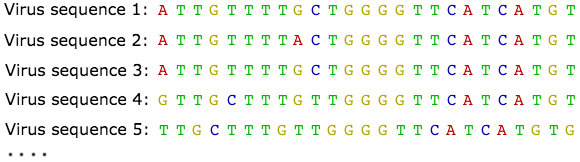
\includegraphics[width=0.7\linewidth]{FluSequence0.png}}
\caption{A list of unaligned nucleotide sequences.}
\label{sequences}
\end{figure}

\vspace{2mm}
\noindent{However, in real analyses the sequences are much longer than shown in Figure 1 - (in fact, they must be, otherwise there is not enough 
information to tell us anything with enough certainty to be useful!) - and also a best alignment may not be all that obvious.}

\vspace{2mm}
\noindent{How do we go about lining up these sequences?}

\vspace{2mm}
[ROSALIND problems:  ``Counting DNA nucleotides" and ``Finding a Motif in DNA"]

\subsection{Building a tree}



\section{The Dynamics of Epidemics}

\subsection{SI, SIS, and SIR models}

\section{Phylodynamics}

\subsection{Sequences to SIR model}

\subsection{Phylodynamics in BEAST 2}

%----------------------------------------------------------------------------------------
%	BIBLIOGRAPHY
%----------------------------------------------------------------------------------------
\newpage
\begin{thebibliography}{99} % Bibliography - this is intentionally simple in this template

%\bibitem[{{Vaughan and Drummond\/}, 2013}]{MASTER}
%{\sc Vaughan, T.~G.} and {\sc A.~J. Drummond}, 2013.
%A Stochastic Simulator of Birth–Death Master Equations with Application to Phylodynamics.
%\newblock Mol. Biol. Evol.
 
\end{thebibliography}

%----------------------------------------------------------------------------------------
\end{document}